\input{preamble.tex}
\author{José Miguel Saavedra Aguilar}
\title{Tarea 08}
\begin{document}

\pagestyle{plain}

\setlength{\parskip}{10pt}
\setlength{\parindent}{5pt}
\begin{minipage}{0.2\linewidth}
\vspace{-1cm}
\includegraphics[width=0.9\linewidth]{logoCIMAT11.png}
\end{minipage}
\begin{minipage}{0.7\linewidth}
\vspace{-1cm}
\noindent {\large \color{cimatred}\textbf{Centro de Investigación en Matemáticas, A.C.}}\\
\textbf{Métodos Numéricos}
\end{minipage}
\vspace{-5mm}
\begin{center}
\textbf{\large \thetitle}\\   %TITULO
\vspace{3mm}
\theauthor
\end{center}
\vspace{-5mm}
\rule{\linewidth}{0.1mm}

\begin{abstract}
En esta tarea se exploran los métodos de mínimos cuadrados y de interpolación para aproximar funciones a través de observaciones.
\end{abstract}
\section{Metodología}
\subsection{Método de Mínimos Cuadrados}
Sea $f:\R\to \R$ una función real, $x\in\R^{m}$ y $g:\R\to\R^{n}$ tal que $g(x)=\bigl( g_1(x), \ldots, g_n(x) \bigr)$ y $n\leq m$. Queremos aproximar $f\approx \alpha^{\top} g$, para $\alpha \in \R^n$. El Error Cuadrático Medio se define como:
\begin{align*}
ECM(\alpha)&=\frac{1}{m}\sqrt{\sum\limits_{i=1}^m \bigl(f(x_i)- \alpha^{\top}g(x_i)\bigr)^2}
\end{align*}
Definimos $y\in \R^m$ y $G\in R^{m\times n}$ tales que $y_i=f(x_i)$ y $G_{i,j}=g_j(x_i)$. Entonces, el Error Cuadrático Medio está dado por:
\begin{align*}
ECM(\alpha)&=\frac{1}{m}\norm{y-G\alpha}_2
\end{align*}
Para obtener el valor $\alpha^*$ que minimiza el Error Cuadrático Medio, derivamos con respecto de $\alpha$:
\begin{align*}
\nabla_{\alpha} ECM(\alpha^*)&= \frac{\nabla_{\alpha} \left(y-G\alpha\right)^{\top}\left(y-G\alpha\right)}{2m \norm{y-G\alpha^*}_2}\\
\nabla_{\alpha} ECM(\alpha^*)&= \frac{1}{m \norm{y-G\alpha^*}_2}G^{\top}\left(y-G\alpha^*\right)\\
\nabla_{\alpha} ECM(\alpha^*)&= \frac{1}{m \norm{y-G\alpha^*}_2}G^{\top}y-G^{\top}G\alpha^*
\end{align*}
Por las condiciones necesarias de primer orden\cite{Nocedal2006}, los puntos críticos de $ECM(\alpha)$ cumplen $\nabla_\alpha ECM(\alpha^*)=0$, de donde tenemos que $\alpha^*$ es la única solución de:
\begin{align*}
G^{\top}G\alpha^*&=G^{\top}y
\end{align*}
Además, notamos que
\begin{align*}
\nabla_{\alpha}^2 ECM(\alpha)&=\nabla_{\alpha}\left( \frac{1}{m \norm{y-G\alpha}_2}\right) \left(y-G^{\top}G\alpha\right) + \frac{1}{m \norm{y-G\alpha}_2} G^{\top}G\\
\nabla_{\alpha}^2 ECM(\alpha^*)&=\frac{1}{m \norm{y-G\alpha^*}_2} G^{\top}G
\end{align*}
Una vez que $\nabla_{\alpha}^2 ECM(\alpha^*)$ es simétrica y positiva definida siempre que $\mathrm{rango}(G)=n$, las condiciones suficientes de segundo orden garantizan que $\alpha^*$ minimiza el Error Cuadrático Medio.
\subsubsection{Polinomios}
Supongamos que queremos aproximar $f$ con un polinomio de grado $n$ para $n<m$, entonces $g(x)=\bigl(1,x,\ldots,x^n \bigr)$, de forma que:
\begin{align*}
G&=\begin{pmatrix}
1 & x_1 & \cdots & x_1^n\\
1 & x_2 & \cdots & x_2^n\\
\vdots & \vdots & \ddots & \vdots\\
1 & x_i & \cdots & x_i^n\\
\vdots & \vdots & \ddots & \vdots\\
1 & x_m & \cdots & x_m^n
\end{pmatrix}
\end{align*}
Por ejemplo, si $n=1$, es decir, una aproximación lineal de $f$,
\begin{align*}
G&=\begin{pmatrix}
1 & x_1\\
1 & x_2\\
\vdots & \vdots\\
1 & x_i \\
\vdots & \vdots\\
1 & x_m
\end{pmatrix}.
\end{align*}
\subsection{Interpolación}
Sea $x\in \R^m$ y $f:\R\to\R$. Buscamos un polinomio $p$ de grado $m-1$ tal que $p(x_i)=f(x_i)$ para $i=1,\ldots,m$. Una forma de calcularlo es por mínimos cuadrados, donde $G$ tendrá la forma:
\begin{align*}
G&=\begin{pmatrix}
1 & x_1 & \cdots & x_1^{m-1}\\
1 & x_2 & \cdots & x_2^{m-1}\\
\vdots & \vdots & \ddots & \vdots\\
1 & x_i & \cdots & x_i^{m-1}\\
\vdots & \vdots & \ddots & \vdots\\
1 & x_m & \cdots & x_m^{m-1}
\end{pmatrix}
\end{align*}
Una vez que $G$ es cuadrada y de rango completo, $G^{-\top}$ existe, por lo que $\alpha^*$ esta dado por:
\begin{align*}
G\alpha^*&=y
\end{align*}
Así, el polinomio está dado por
\begin{align*}
p(x)=\alpha_1 + \alpha_2 x + \ldots + \alpha_{m}x^{m-1}
\end{align*}
\subsubsection{Polinomios de Lagrange}
Otra representación del polinomio de grado $m-1$ que cumpla $p(x_i)=f(x_i)$ para $i=1,\ldots,m$ fue propuesta por Lagrange. Esta representación está dada por
\begin{align*}
p(x)&=\sum\limits_{i=1}^{m}f(x_i)l_i(x),
\end{align*}
donde $l_i$ se conocen como los factores de Lagrange, y se calculan de la forma\cite{Kress2012}:
\begin{align*}
l_i(x)&=\prod\limits_{k\not =i}\frac{x-x_k}{x_i-x_k}, & i&=1,\ldots, m
\end{align*}
Nótese que los factores de Lagrange son polinomios de grado $m-1$ tales que $l_i(x_i)=1$ y $l_i(x_j)=0$ para $j\not =i$. Así, tenemos que $p(x_i)=f(x_i)$ para $i=1,\ldots,m$.
\subsubsection{Polinomios de Newton}
En 1676, Newton obtuvo una representación del polinomio $p$ que cumple $p(x_i)=f(x_i)$ para $i=1,\ldots,m$. Para obtenerla, se deben calcular las llamadas \textit{diferencias divididas}. La diferencia dividida de orden $k$ se define por:
\begin{align*}
D_j^k&:=\begin{cases} f(x_j) & k=0\\
\frac{D_{j+1}^{k-1}-D_{j}^{k-1}}{x_{j+k}-x_j}& k=1,\ldots,m-1 \end{cases}
\end{align*}
para $j=1,\ldots,m-k$. Así, el polinomio está dado por\cite{Kress2012}
\begin{align*}
p(x)&=f(x_1) + \sum\limits_{k=1}^{m-1} D_{1}^{k+1} \prod\limits_{i=1}^{k}(x-x_i)
\end{align*}
Nótese que $p(x_1)=f(x_1)$ y que
\begin{align*}
p(x_{j})-p(x_{j-1})&=\sum\limits_{k=2}^j D_{1}^k \prod\limits_{i=1}^{k-1}(x_j-x_i) - \sum\limits_{k=2}^{j-1} D_{1}^k \prod\limits_{i=1}^{k-1}(x_{j-1}-x_i)\\
p(x_{j})-p(x_{j-1})&=\sum\limits_{k=2}^j D_{1}^k (x_j-x_{j-1})\\
p(x_{j})-p(x_{j-1})&=D_{j}^1 -D{j-1}^1\\
p(x_{j})-p(x_{j-1})&=f(x_j) - f(x_{j-1}^1)\\
p(x_{j})&=f(x_j)
\end{align*}
\section{Pseudocódigo}

\begin{algorithm}[H]
	\SetAlgoLined
	\KwIn{$x,y$}
	\KwOut{$\alpha$}
	\For{$i=1$ \textbf{hasta} $m$}{
		$G_{i,1}\gets 1$\;
		$G_{i,2}\gets x_i$\;
	}
	$A\gets G^{\top}G$\;
	$b\gets G^{\top}y$\;
	\textbf{resolver} $A\alpha=b$\;
  \caption{Método de mínimos cuadrados para aproximación lineal.}\label{alg:minimosCuadradosLineal}
\end{algorithm}

\begin{algorithm}[H]
	\SetAlgoLined
	\KwIn{$x,y,n$}
	\KwOut{$\alpha$}
	\For{$i=1$ \textbf{hasta} $m$}{
		\For{$j=1$ \textbf{hasta} $n+1$}{
			$G_{i,j}\gets x_i^{j-1}$\;
		}
	}
	$A\gets G^{\top}G$\;
	$b\gets G^{\top}y$\;
	\textbf{resolver} $A\alpha=b$\;
  \caption{Método de mínimos cuadrados para un polinomio de grado $n$.}\label{alg:minimosCuadradosPolinomial}
\end{algorithm}

\begin{algorithm}[H]
	\SetAlgoLined
	\KwIn{$x,y,g$}
	\KwOut{$\alpha$}
	\For{$i=1$ \textbf{hasta} $m$}{
		\For{$j=1$ \textbf{hasta} $n$}{
			$G_{i,j}\gets g_j(x_i)$\;
		}
	}
	$A\gets G^{\top}G$\;
	$b\gets G^{\top}y$\;
	\textbf{resolver} $A\alpha=b$\;
  \caption{Método de mínimos cuadrados para funciones $g_1, \ldots, g_n$ dadas.}\label{alg:minimosCuadrados}
\end{algorithm}

\begin{algorithm}[H]
	\SetAlgoLined
	\KwIn{$z,x,y$}
	\KwOut{$p(z)$}
	\For{$i=1$ \textbf{hasta} $m$}{
		\For{$j=1$ \textbf{hasta} $m$}{
			$G_{i,j}\gets x_i^{j-1}$\;
		}
	}
	\textbf{resolver} $G\alpha=y$\;
	$p(z)\gets \sum\limits_{i=1}^m \alpha_iz^{i-1}$
  \caption{Método de mínimos cuadrados para interpolar un polinomio por $m$ puntos.}\label{alg:interpolacionPolinomial}
\end{algorithm}

\begin{algorithm}[H]
	\SetAlgoLined
	\KwIn{$z,x,y$}
	\KwOut{$p(z)$}
	$p(z)\gets 0$\;
	\For{$i=1$ \textbf{hasta} $m$}{
		$l_i\gets\prod\limits_{k\not =i}\frac{z-x_k}{x_i-x_k}$\;
		$p(z)\gets p(z) + y_il_i$\;
	}
  \caption{Método de Lagrange para interpolar un polinomio por $m$ puntos.}\label{alg:polinomioLagrange}
\end{algorithm}

\begin{algorithm}[H]
	\SetAlgoLined
	\KwIn{$z,x,y$}
	\KwOut{$p(z)$}
	$D^0\gets y$\;
	\For{$k=1$ \textbf{hasta} $m-1$}{
		\For{$j=1$ \textbf{hasta} $m-k$}{
			$D_j^k\gets\frac{D_{j+1}^{k-1}-D_{j}^{k-1}}{x_{j+k}-x_j}$\;
		}
	}
	$p(z)\gets y_1$\;
	\For{$k=1$ \textbf{hasta} $m-1$}{
		$p(z)\gets p(z) + D_{1}^{k+1} \prod\limits_{i=1}^{k}(z-x_i)$
	}
  \caption{Método de Newton para interpolar un polinomio por $m$ puntos.}\label{alg:polinomioNewton}
\end{algorithm}

\section{Algoritmos}
Para ejecutar los algoritmos simplemente se debe correr la siguiente linea desde la Terminal:
\begin{center}
\texttt{julia main.jl}
\end{center}
desde la carpeta del problema. A continuación se muestra la ejecución de los algoritmos para los problemas de la tarea.\\
\begin{figure}[H]
\centering
\includegraphics[scale=0.8]{p1a.jpg}
\caption{Ejecución del algoritmo \ref{alg:minimosCuadradosLineal}}
\end{figure}
\begin{figure}[H]
\centering
\includegraphics[scale=0.8]{p1b.jpg}
\caption{Ejecución del algoritmo \ref{alg:minimosCuadradosPolinomial}}
\end{figure}
\begin{figure}[H]
\centering
\includegraphics[scale=0.8]{p1c.jpg}
\caption{Ejecución del algoritmo \ref{alg:minimosCuadrados}}
\end{figure}
\begin{figure}[H]
\centering
\includegraphics[scale=0.8]{p2a.jpg}
\caption{Ejecución del algoritmo \ref{alg:interpolacionPolinomial}}
\end{figure}
\begin{figure}[H]
\centering
\includegraphics[scale=0.8]{p2b.jpg}
\caption{Ejecución del algoritmo \ref{alg:polinomioLagrange}}
\end{figure}
\begin{figure}[H]
\centering
\includegraphics[scale=0.8]{p2c.jpg}
\caption{Ejecución del algoritmo \ref{alg:polinomioNewton}}
\end{figure}
Para el ejercicio 3, es necesario instalar las librerías \texttt{Plots.jl} y \texttt{LaTeXStrings}, por lo que si no se tienen instalados, se incluye un script que las instala:
\begin{center}
\texttt{julia runFirst.jl}\\
\texttt{julia main.jl}
\end{center}
\begin{figure}[H]
\centering
\includegraphics[scale=0.8]{p3.jpg}
\caption{Ejecución del ejercicio 3}
\end{figure}

\section{Resultados}
Se consideraron las funciones:
\begin{align*}
f_1(x)&=\frac{1}{1+25x^2},\\
f_2(x)&=\abs{x}-\frac{x}{2}-x^2
\end{align*}
Para los algoritmos \ref{alg:minimosCuadradosLineal}, \ref{alg:minimosCuadradosPolinomial} y \ref{alg:minimosCuadrados} se consideran diferentes tamaños de $m$, $n=6$ para \ref{alg:minimosCuadradosPolinomial}, $g_1(x)$ para \ref{alg:minimosCuadrados} de $f_1$ y $g_2(x)$ para \ref{alg:minimosCuadrados} de $f_2(x)$, donde
\begin{align*}
g_1(x)&=\begin{pmatrix}
1\\
e^{-x^2}\\
\cos(\pi x)
\end{pmatrix}, &
g_2(x)&=\begin{pmatrix}
x\\
e^{-x^2}\\
\cos(2\pi x)
\end{pmatrix}.
\end{align*}
Los resultados para los métodos de mínimos cuadrados para $f_1$ considerando $m=5$, $m=100$ y $m=1000$ están en la tabla \ref{tab:minimosCuadrados1}. Las interpolaciones resultantes se encuentran en la figura \ref{fig:minimosCuadrados1}.\par
\begin{table}[H]
\centering
\begin{tabular}{|c|c|c|c|}
\hline
$m$  & lineal      & polinomial  & $g_1(x)$    \\ \hline
5    & 1.69131E-01 & 7.26000E-15 & 2.37836E-02 \\ \hline
100  & 2.83819E-02 & 8.30105E-03 & 4.23777E-03 \\ \hline
1000 & 8.57970E-03 & 2.68657E-03 & 3.70063E-03 \\ \hline
\end{tabular}
\caption{Resultados de mínimos cuadrados para $f_1(x)$}
\label{tab:minimosCuadrados1}
\end{table}
\begin{figure}[H]
\centering
\begin{subfigure}[b]{0.3\textwidth}
	\centering
	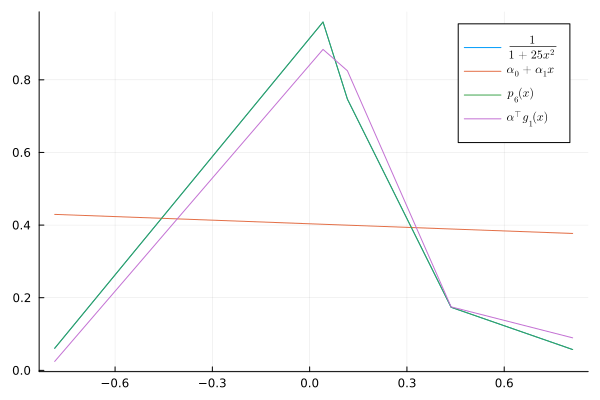
\includegraphics[width=\textwidth]{pMinimosCuadrados1-5.png}
	\caption{$m=5$}
\end{subfigure}
\hfill
\begin{subfigure}[b]{0.3\textwidth}
	\centering
	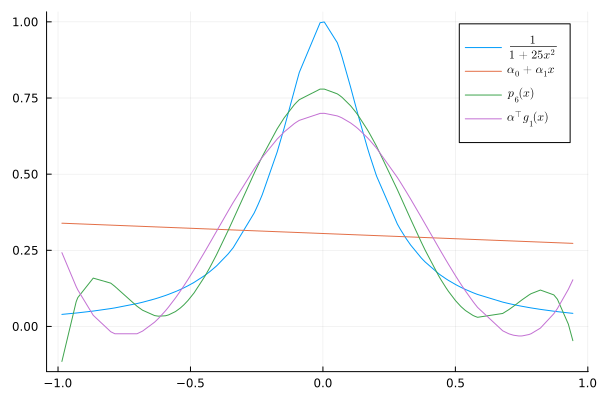
\includegraphics[width=\textwidth]{pMinimosCuadrados1-100.png}
	\caption{$m=100$}
\end{subfigure}
\hfill
\begin{subfigure}[b]{0.3\textwidth}
	\centering
	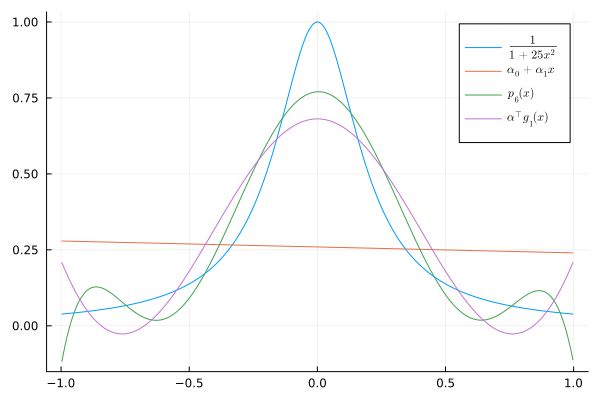
\includegraphics[width=\textwidth]{pMinimosCuadrados1-1000.png}
	\caption{$m=1000$}
\end{subfigure}
\caption{Mínimos cuadrados de $f_1$ para distintos valores de $m$}
\label{fig:minimosCuadrados1}
\end{figure}
Así también, los resultados para los métodos de mínimos cuadrados para $f_2$ considerando $m=5$, $m=100$ y $m=1000$ están en la tabla \ref{tab:minimosCuadrados2}. Las interpolaciones resultantes se observan en la figura \ref{fig:minimosCuadrados2}.\par
\begin{table}[H]
\centering
\begin{tabular}{|c|c|c|c|}
\hline
$m$  & lineal      & polinomial  & $g_1(x)$    \\ \hline
5    & 3.04502E-02 & 5.43616E-16 & 2.74856E-02 \\ \hline
100  & 7.01255E-03 & 2.17782E-03 & 4.23777E-03 \\ \hline
1000 & 2.31023E-03 & 6.92983E-04 & 1.46028E-03 \\ \hline
\end{tabular}
\caption{Resultados de mínimos cuadrados para $f_2(x)$}
\label{tab:minimosCuadrados2}
\end{table}
\begin{figure}[H]
\centering
\begin{subfigure}[b]{0.3\textwidth}
	\centering
	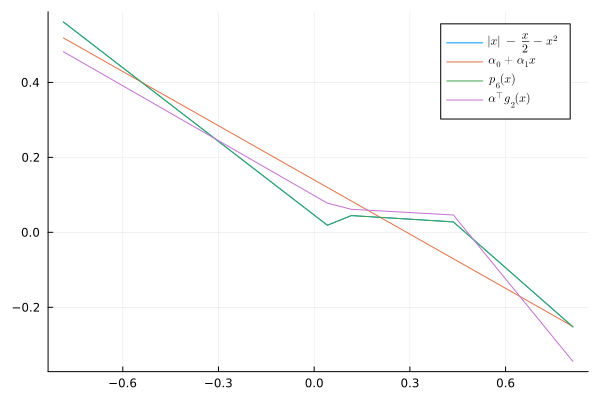
\includegraphics[width=\textwidth]{pMinimosCuadrados2-5.png}
	\caption{$m=5$}
\end{subfigure}
\hfill
\begin{subfigure}[b]{0.3\textwidth}
	\centering
	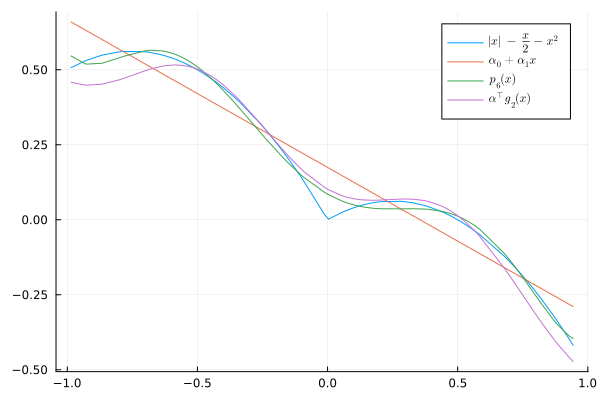
\includegraphics[width=\textwidth]{pMinimosCuadrados2-100.png}
	\caption{$m=100$}
\end{subfigure}
\hfill
\begin{subfigure}[b]{0.3\textwidth}
	\centering
	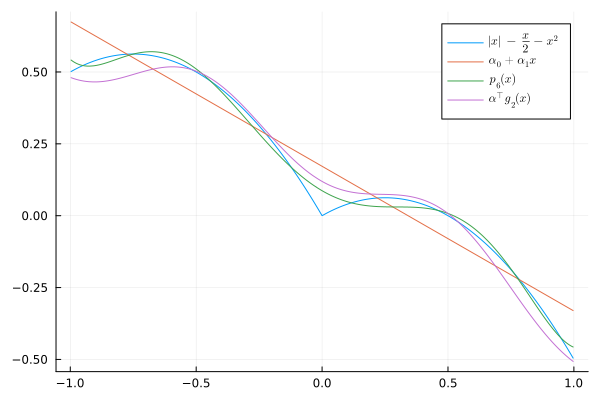
\includegraphics[width=\textwidth]{pMinimosCuadrados2-1000.png}
	\caption{$m=1000$}
\end{subfigure}
\caption{Mínimos cuadrados de $f_2$ para distintos valores de $m$}
\label{fig:minimosCuadrados2}
\end{figure}
Para los algoritmos de interpolación por polinomios, se consideran $n$ puntos aleatorios en $(-1,1)$ y $m=1000$ puntos aleatorios para evaluar $p(x)$ dado por los algoritmos \ref{alg:interpolacionPolinomial}, \ref{alg:polinomioLagrange} y \ref{alg:polinomioNewton}, para $n=3$, $n=5$ y $n=8$. Como era de esperarse, el polinomio es idéntico para los tres algoritmos. El Error Cuadrático Medio considerando los 1000 puntos que se evaluan se encuentran en la tabla \ref{tab:interpolacion}. Las interpolaciones para $f_1$ se pueden observar en la figura \ref{fig:interpolacion1}. mientras que las de $f_2$ en la figura \ref{fig:interpolacion2}.
\begin{table}[H]
\centering
\begin{tabular}{|c|c|c|}
\hline
$n$  & $f_1$       & $f_2$       \\ \hline
5    & 4.33957E-02 & 9.77907E-03 \\ \hline
100  & 9.23096E-02 & 1.93744E-02 \\ \hline
1000 & 1.39590E-01 & 2.60778E-02 \\ \hline
\end{tabular}
\caption{Resultados de aproximación por interpolación}
\label{tab:interpolacion}
\end{table}
\begin{figure}[H]
\centering
\begin{subfigure}[b]{0.3\textwidth}
	\centering
	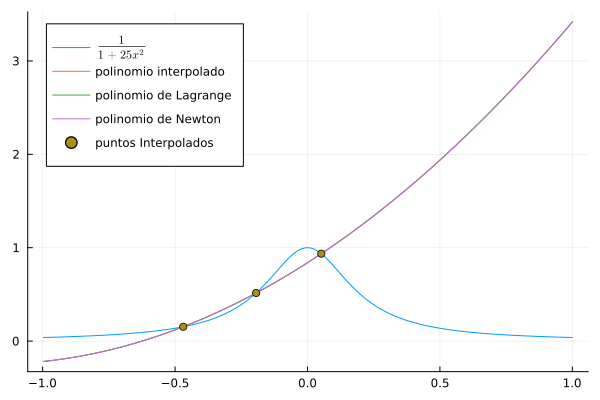
\includegraphics[width=\textwidth]{pInterpolacion1-3.png}
	\caption{$m=5$}
\end{subfigure}
\hfill
\begin{subfigure}[b]{0.3\textwidth}
	\centering
	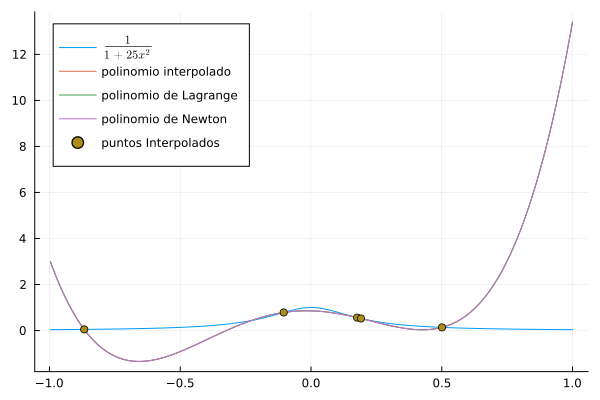
\includegraphics[width=\textwidth]{pInterpolacion1-5.png}
	\caption{$m=100$}
\end{subfigure}
\hfill
\begin{subfigure}[b]{0.3\textwidth}
	\centering
	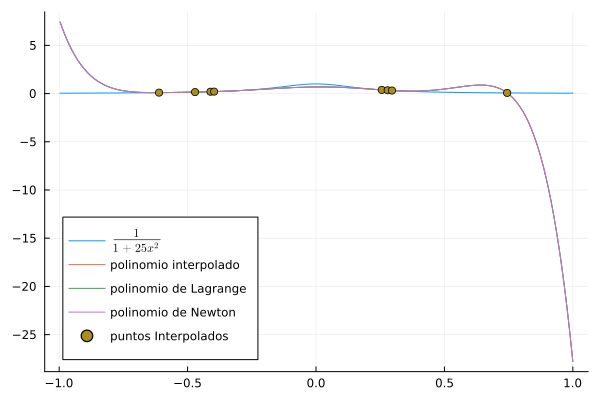
\includegraphics[width=\textwidth]{pInterpolacion1-8.png}
	\caption{$m=1000$}
\end{subfigure}
\caption{Interpolación sobre $n$ puntos aleatorios de $f_1$}
\label{fig:interpolacion1}
\end{figure}
\begin{figure}[H]
\centering
\begin{subfigure}[b]{0.3\textwidth}
	\centering
	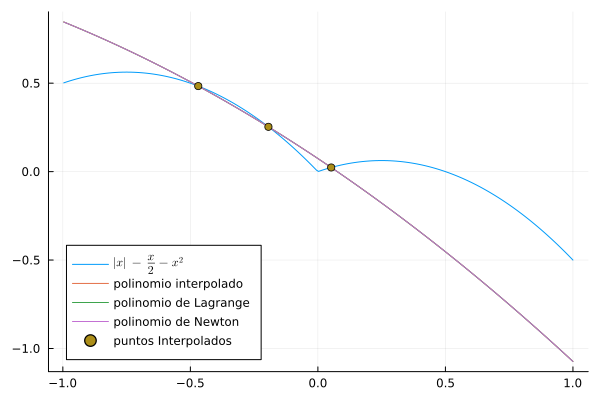
\includegraphics[width=\textwidth]{pInterpolacion2-3.png}
	\caption{$m=5$}
\end{subfigure}
\hfill
\begin{subfigure}[b]{0.3\textwidth}
	\centering
	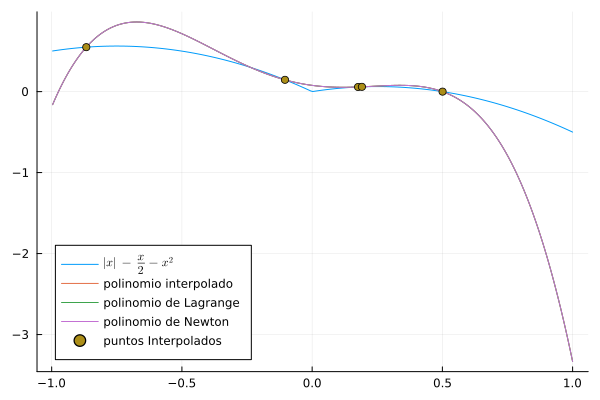
\includegraphics[width=\textwidth]{pInterpolacion2-5.png}
	\caption{$m=100$}
\end{subfigure}
\hfill
\begin{subfigure}[b]{0.3\textwidth}
	\centering
	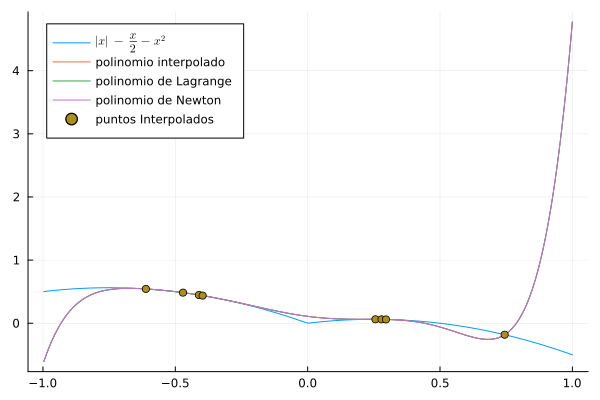
\includegraphics[width=\textwidth]{pInterpolacion2-8.png}
	\caption{$m=1000$}
\end{subfigure}
\caption{Interpolación sobre $n$ puntos aleatorios de $f_1$}
\label{fig:interpolacion2}
\end{figure}
\section{Conclusiones}
Notamos que los métodos de mínimos cuadrados son mejores para aproximar funciones pues minimizan el Error Cuadrático Medio para el intervalo completo, mientras que interpolación solo garantiza que $n$ puntos coincidan con la solución exacta. Además, notamos que tomar puntos aleatorios para la interpolación no es la mejor estrategia, pues es posible que no se cubran los extremos del intervalo de nuestro interés. Además, mientras tomamos $n$ más grandes, nuestra aproximación tiene mayores oscilaciones, pues el grado del polinomio crece.
\bibliography{biblio}
\bibliographystyle{IEEEtranS}
\end{document}